\documentclass[11pt]{amsart}
\usepackage{amsmath,amsthm,amssymb,mathrsfs,amsfonts,verbatim,enumitem,color,leftidx}
\usepackage{tikz}
\usepackage{pgfmath}
\usepackage[colorlinks]{hyperref}
\usepackage{tikz}
\usetikzlibrary{arrows,snakes,backgrounds}

\begin{document}

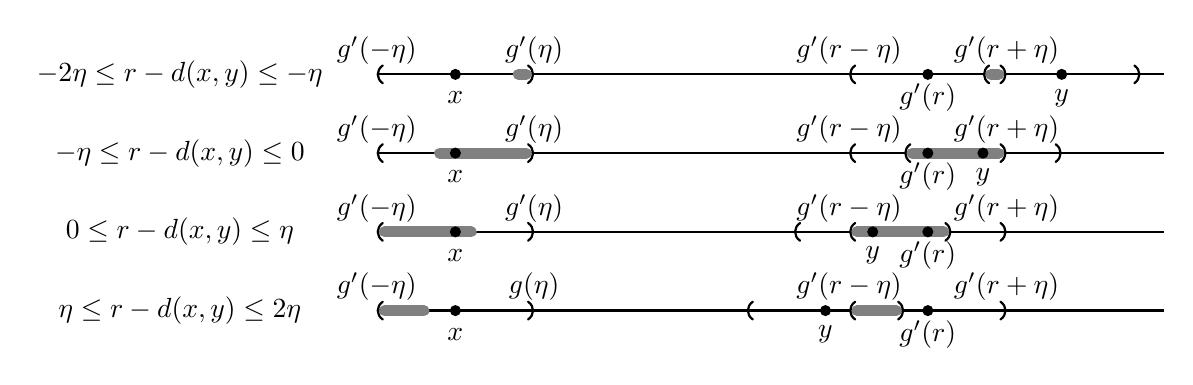
\begin{tikzpicture}[scale=1]
\draw [thick](-4,4)--(6,4);\draw [thick](-4,3)--(6,3);\draw [thick](-4,2)--(6,2);\draw [thick](-4,1)--(6,1);
\draw [thick,(-)](-4,4)--(-2,4);\draw [thick,(-)](-4,3)--(-2,3);\draw [thick,(-)](-4,2)--(-2,2);\draw [thick,(-)](-4,1)--(-2,1);
\draw [thick,(-)](2,4)--(4,4);\draw [thick,(-)](2,3)--(4,3);\draw [thick,(-)](2,2)--(4,2);\draw [thick,(-)](2,1)--(4,1);
\draw[thick,(-)](3.7,4)--(5.7,4);\draw[thick,(-)](2.7,3)--(4.7,3);\draw[thick,(-)](1.3,2)--(3.3,2);\draw[thick,(-)](0.7,1)--(2.7,1);
\draw[line cap=round,line width=4pt, color=gray](-2.2,4)--(-2.1,4);\draw[line cap=round,line width=4pt, color=gray](-3.9,2)--(-2.8,2);\draw[line cap=round,line width=4pt, color=gray](-3.2,3)--(-2.1,3);\draw[line cap=round,line width=4pt, color=gray](-3.4,1)--(-3.9,1);
\draw[line cap=round,line width=4pt, color=gray](3.8,4)--(3.9,4);\draw[line cap=round,line width=4pt, color=gray](2.8,3)--(3.9,3);\draw[line cap=round,line width=4pt, color=gray](2.1,2)--(3.2,2);\draw[line cap=round,line width=4pt, color=gray](2.1,1)--(2.6,1);
\fill (-3,4)  circle (2pt);\fill (-3,3)    circle (2pt);\fill (-3,2)    circle (2pt);\fill (-3,1)    circle (2pt);
\fill (3,4)    circle (2pt);\fill (3,3)    circle (2pt);\fill (3,2)    circle (2pt);\fill (3,1)    circle (2pt);
\fill (4.7,4)    circle (2pt);\fill (3.7,3)    circle (2pt);\fill (2.3,2)    circle (2pt);\fill (1.7,1)    circle (2pt);
\node at (-6.5,4) {$-2\eta \leq r-d(x,y) \leq -\eta$};\node at (-3,3.7) {$x$};\node at (3,3.7) {$g'(r)$};\node at (4.7,3.7) {$y$};\node at (-4,4.3) {$g'(-\eta)$};\node at (-2,4.3) {$g'(\eta)$};\node at (2,4.3) {$g'(r-\eta)$};\node at (4,4.3) {$g'(r+\eta)$};
\node at (-6.5,3) {$-\eta \leq r-d(x,y) \leq 0$};\node at (-3,2.7) {$x$};\node at (3,2.7) {$g'(r)$};\node at (3.7,2.7) {$y$};\node at (-4,3.3) {$g'(-\eta)$};\node at (-2,3.3) {$g'(\eta)$};\node at (2,3.3) {$g'(r-\eta)$};\node at (4,3.3) {$g'(r+\eta)$};
\node at (-6.5,2) {$0 \leq r-d(x,y) \leq \eta$};\node at (-3,1.7) {$x$};\node at (3,1.7) {$g'(r)$};\node at (2.3,1.7) {$y$};\node at (-4,2.3) {$g'(-\eta)$};\node at (-2,2.3) {$g'(\eta)$};\node at (2,2.3) {$g'(r-\eta)$};\node at (4,2.3) {$g'(r+\eta)$};
\node at (-6.5,1) {$\eta \leq r-d(x,y) \leq 2\eta$};\node at (-3,0.7) {$x$};\node at (3,0.7) {$g'(r)$};\node at (1.7,0.7) {$y$};\node at (-4,1.3) {$g'(-\eta)$};\node at (-2,1.3) {$g(\eta)$};\node at (2,1.3) {$g'(r-\eta)$};\node at (4,1.3) {$g'(r+\eta)$};
\end{tikzpicture}

\end{document}